\section{Setup Environment}

We simulate all path-finding processes based on the framework of
GridWorld\cite{web:gridworld}, an AP case study project from CollegeBoard
\footnote{https://www.collegeboard.org/}. It provides graphical user interface
based on Java AWT where visual objects can interact and perform customized
actions in a two-dimensional grid map. In the next part, we will first
illustrate original GridWorld framework and our enhancement of displaying
colored path. 

\subsection{GridWorld Architecture and Modification}

The source code of original GridWorld project is placed in $src/main/framework$
folder and its structure can be divided into four parts, as shown in Figure 
\ref{fig:framework-structure}.

\begin{figure}[ht]
  \centering
  \begin{subfigure}[b]{0.45\textwidth}
    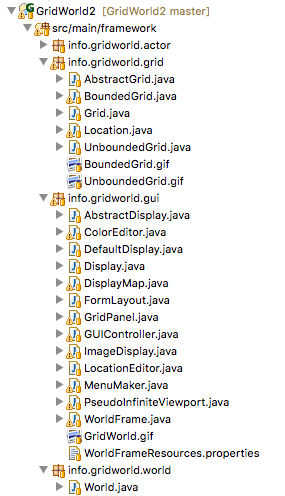
\includegraphics[width=0.9\textwidth]{framework-structure}
    \caption{GridWorld structure}
    \label{fig:framework-structure}
  \end{subfigure}
  ~
  \begin{subfigure}[b]{0.46\textwidth}
    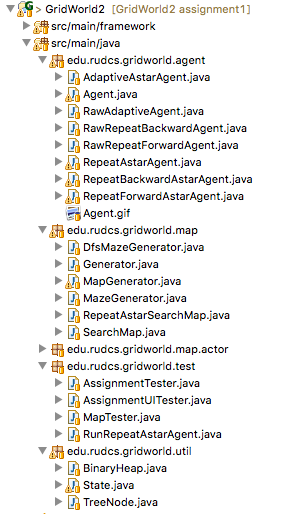
\includegraphics[width=0.9\textwidth]{project-structure}
    \caption{Project structure}
    \label{fig:project-structure}
  \end{subfigure}
\caption{Structure of GridWorld framework and path-finding project}
\end{figure}

The $actor$ package contains objects whose behavior on the map can be arbitrarily 
defined by rewriting $act$ method in each inherited class:

\begin{lstlisting}
%%@Override%%
public void act()
\end{lstlisting}

The $grid$ package defines features on bounded and unbounded grid map as well 
as connections between map and actors. The $gui$ package encapsulates low-level
Java AWT to provide APIs for visualization and interactions of map and actors.
The $world$ package provides high-level integration of actors and world.

In order to visualize the presumed unblocked path and the set of nodes expanded
and explored after each planning, we enhance the $GridPanel$ class in the 
GUI package by implementing the method below:

\begin{lstlisting}
private void drawColoredLocations(Graphics2D g2)
\end{lstlisting}

Meanwhile, following five abstract methods related to colored grid are added 
to $Grid$ interface and classes like $BoundedGrid$ and $UnboundedGrid$ are 
responsible to implement color configuration on each grid.

\begin{lstlisting}
ArrayList<Location> getColoredLocations();
Color getColor(Location loc);
void putColor(Location loc, Color color);
void removeColor(Location loc);
void resetColors();
\end{lstlisting}

The source code related to assignment is placed in $src/main/java$ folder, as 
shown in Figure \ref{fig:project-structure}, which are divided into five packages.
The $agent$ package defines the simulated agents equipped with specific navigation 
algorithm for solving goal-directed path-finding problem. The $map$ package 
provides APIs for generation of random map and corridor-like maze. The $map.actor$ 
package defines some static object on the map like obstacles and goal. The $test$
package contains simulation program for experiment and testing. The $util$
package includes some self-defined data structures to be used in storing 
intermediate result of algorithm.

\subsection{Data Structures}

In the project, we implement some useful data structures from scratch, like
binary heap and tree, by referring to CLRS\cite{clrs}. The detailed interfaces
provided by these data structures are listed in Figure \ref{fig:ds}.

\begin{figure}[ht!]
  \centering
  \begin{subfigure}[b]{0.45\textwidth}
    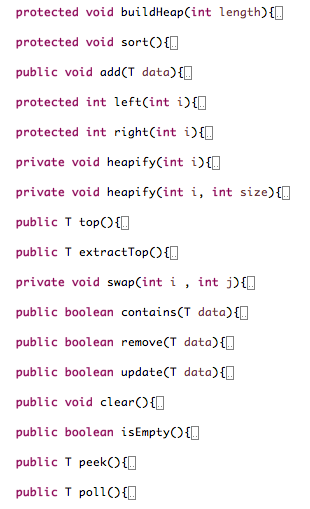
\includegraphics[width=\textwidth]{binaryheap}
    \caption{Interfaces for Binary Heap}
  \end{subfigure}
  ~
  \begin{subfigure}[b]{0.45\textwidth}
    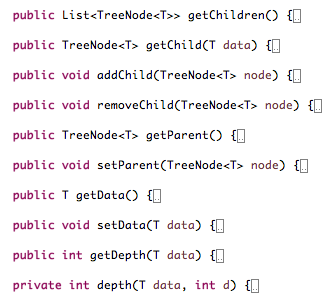
\includegraphics[width=\textwidth]{tree}
    \caption{Interfaces for Tree}
  \end{subfigure}
\caption{Interfaces of Data Structures}
\label{fig:ds}
\end{figure}

\subsection{How to Run}

Our project is built and packed by Gradle\footnote{http://gradle.org/}, 
an open-source build automation tool. To run the project, you should first 
install and setup Gradle environment on your computer, and install Gradle plugin 
for Eclipse, called "Gradle Integration for Eclipse". Then, download complete 
source code of the project, which is attached in Sakai or available on the 
Github (\url{https://github.com/orcax/GridWorld2}). Finally, inside Eclipse,
click $File\rightarrow Import\rightarrow Gradle\rightarrow Gradle~Project$ to
import project. All runnable programs are placed in $test$ package.

\subsection{Maze Generation Algorithm}

In the experiment, we mainly use two kinds of grid map, namely random map with
discrete obstacles and random maze with consecutive obstacles. The random map
is generated according to the assignment requirement, so for each map, there
are about 30\% obstacles and 70\% roads. The start position and the goal
position can be placed either randomly or on diagonal corners. Difference
between these two ways lies in the absolute distance between start and goal,
although, the experimental result implies that this initial distance in this
type of random map has nearly no influence on the performance of three
algorithms. So in this case, we simply collect maps that exist a path between
the start position and goal position.

Random maze is the other type of map tested in the experiment. It is generated
according to DFS by expanding neighbors randomly. The generation process is 
described as Algorithm \ref{alg:maze-gen}.

\begin{algorithm}[ht!]
\caption{Maze Generation Algorithm by DFS}
\label{alg:maze-gen}
\begin{algorithmic}[1]
\Function{Generate-By-Dfs}{$map$}
  \State set all cells in $map$ as $WALL$
  \State $r=random(\lfloor map.rows/2 \rfloor) * 2 + 1$
  \State $c=random(\lfloor map.cols/2 \rfloor) * 2 + 1$
  \State $map[r][c] = ROAD$
  \State call \textsc{Random-Dfs}($map, r, c$)
  \State $map[1][1] = START$
  \State $map[map.rows-2][map.cols-2] = GOAL$
\EndFunction
\end{algorithmic}
\begin{algorithmic}[1]
\Function{Random-Dfs}{$map$, $row$, $col$}
  \State $(row',col')$=\textsc{Random-Neighbor}$(map, row, col)$
  \While{$(row',col') \neq NULL$}
    \State $map[row'][col']=ROAD$
    \State $map[(row+row')/2][(col+col')/2]=ROAD$
    \State call \textsc{Random-Dfs}($map, row', col'$)
    \State ($row',col'$)=\textsc{Random-Neighbor}($map, row, col$)
  \EndWhile
\EndFunction
\end{algorithmic}
\begin{algorithmic}[1]
\Function{Random-Neighbor}{$map$, $row$, $col$}
  \State initialize $neighbors$ as empty list
  \If{$row-2 > 0~and~map[row-2][col] \neq ROAD$}
    \State $neighbors$.add($(row-2, col)$)
  \EndIf
  \If{$row+2 < map.rows~and~map[row+2][col] \neq ROAD$}
    \State $neighbors$.add($(row+2, col)$)
  \EndIf
  \If{$col-2 > 0~and~map[row][col-2] \neq ROAD$}
    \State $neighbors$.add($(row, col-2)$)
  \EndIf
  \If{$col+2 < map.cols~and~map[row][col+2] \neq ROAD$}
    \State $neighbors$.add($(row, col+2)$)
  \EndIf
  \Return $neighbors[random(neighbors.size)]$
\EndFunction
\end{algorithmic}
\end{algorithm}

In this algorithm, the map is initialized as two-dimensional array and set 
all cells as obstacles (WALL). Roads will be expanded randomly and paved only 
on the cells of odd index. To generate roads, we first begin with randomly 
picking a cell on the map and set it as road. Then, randomly select one of its 
non-road neighboring nodes (of odd index), set it and the node between them 
as roads. Repeat this procedure until there is no valid neighboring nodes. 
If this happens, traceback to its parent node and do the same thing again. At
last, all nodes of odd index are traversed and some nodes of even index are
set as road to connect two adjacent nodes. Finally, without loss of generality,
we simply set top-left odd bottom-right respectively as start position and goal
position.

It is easy to prove that there is only one depth first tree generated during one 
complete search. The connectivity of single depth first tree make the maze 
always reachable, namely there always exists one path from start to goal. 
Example of two kinds of map of size 50*50 is shown in Figure \ref{fig:map-and-maze}.

\begin{figure}
  \centering
  \begin{subfigure}[b]{0.45\textwidth}
    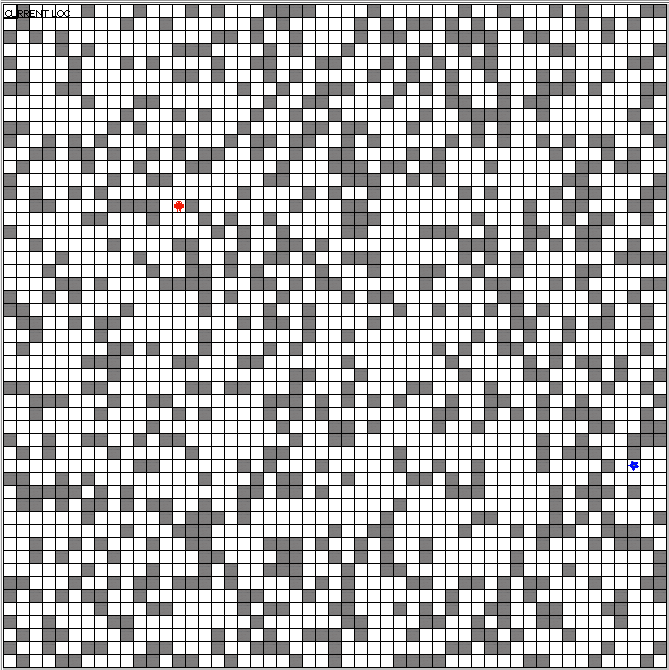
\includegraphics[width=\textwidth]{map.png}
    \caption{Map with discrete obstacles}
  \end{subfigure}
  \begin{subfigure}[b]{0.45\textwidth}
    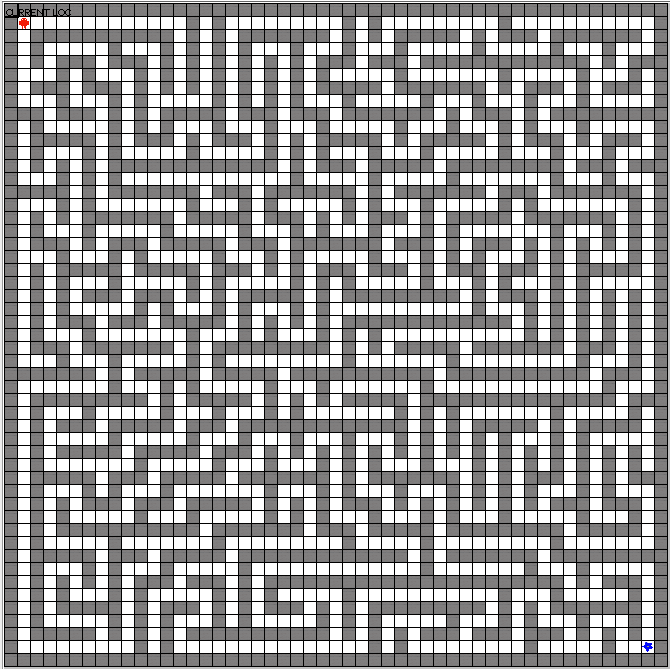
\includegraphics[width=\textwidth]{maze.png}
    \caption{Corridor-like maze}
  \end{subfigure}
  \caption{Example of random map and random maze}
  \label{fig:map-and-maze}
\end{figure}

